% TODO: Procédure d'inscription à l'examen
% TODO: Liste prérequis actu pour les cours optionnels
% TODO: Explication des résultats d'examen
% TODO: Rôle de l'ICA
\documentclass[11pt,french]{article}
	%% Francisation de LaTeX
	\usepackage{babel}
	\usepackage[autolanguage]{numprint}
	\usepackage[utf8]{inputenc}
	\usepackage[T1]{fontenc}
	\usepackage{icomma}
	\usepackage[hidelinks]{hyperref}
	\usepackage{xcolor}
	\hypersetup{
    colorlinks,
    linkcolor={red!50!black},
    citecolor={blue!50!black},
    urlcolor={blue!80!black}}
    \usepackage{graphicx}
    \usepackage{caption}
    \usepackage{wrapfig}
    \usepackage{enumitem}
    \usepackage{lipsum}  % generates filler text

\usepackage{fancyhdr}
\fancyhf{} % clear all header and footers
\renewcommand{\headrulewidth}{0pt} % remove the header rule
\rfoot{\thepage}
\pagestyle{fancy}

\usepackage{epigraph}
% \epigraphsize{\small}% Default
\setlength\epigraphwidth{8cm}
\setlength\epigraphrule{0pt}

\usepackage{etoolbox}

\makeatletter
\patchcmd{\epigraph}{\@epitext{#1}}{\itshape\@epitext{#1}}{}{}
\makeatother

\title{Guide pour les examens professionnels en actuariat}
\author{Antoine Beaupré}



\AtBeginDocument{\def\labelitemi{$\bullet$}}



\begin{document}
\pagenumbering{Roman}
\maketitle
\thispagestyle{fancy}
\begin{abstract}
Ce guide s'adresse en premier lieu aux étudiants qui débutent dans le baccalauréat en actuariat, mais les plus expérimentés y trouveront tout de même de l'information pertinente. Plutôt que de décrire en long et en large le processus d'examens professionnels et les méthodes d'étude à préconiser, ce guide renvoie systématiquement le lecteur vers des pages web en fournissant une brève description de ce qu'on retrouvera à cette adresse.\footnote{Les opinions qui sont exprimées dans ce document n'impliquent en aucun cas l'École d'actuariat, la \emph{Society of Actuaries}, la \emph{Casualty Actuarial Society} ou n'importe quelle autre organisation. Ce document n'est pas non plus une source d'information officielle et devrait seulement être considéré comme un outil de référence.}{\tiny} 
\end{abstract}

\clearpage
\vspace*{\stretch{2}}
\begin{center}
\begin{minipage}{.6\textwidth}
\epigraph{We do not rise to the level of our expectations. We fall to the level of our training.}{--- \textup{Archiloque}, 712-664 av. J.-C.}
\end{minipage}
\end{center}
\vspace{\stretch{3}}
\clearpage

\newpage
\tableofcontents

\newpage
\pagenumbering{arabic}
\setcounter{page}{1}
\section*{Généralités}
\label{sec:generalites}
\addcontentsline{toc}{section}{Généralités}

\subsection*{Les examens professionnels}
\label{subsec:examsprofs}
\addcontentsline{toc}{subsection}{Les examens professionnels}
\captionsetup{justification=centering}
Bien souvent, les examens professionnels sont l'une des premières choses dont l'on entend parler lorsqu'il est question d'actuariat. Il y a beaucoup d'informations disponibles sur le sujet, autant à partir de sources officielles que sur différents forums de discussion.\vspace{\baselineskip}

Afin d'avoir une bonne idée du cheminement, je vous suggère de vous référer en premier lieu aux informations se trouvant sur les sites des deux principales organisations professionnelles en actuariat: la \href{https://soa.org/member/}{\emph{Society of Actuaries (SOA)}} et la \href{http://www.casact.org/}{\emph{Casualty Actuarial Society (CAS)}}. Essentiellement, ce sont leurs champs d'activité différents qui distinguent ces deux organisations; la CAS se spécialise dans l'assurance IARD, alors que la SOA regroupe les branches investissement, gestion de risques en entreprise, assurance-vie, retraite et assurance-maladie.\footnote{ Il est à noter que la spécialisation \emph{General Insurance} de la SOA n'est pas reconnue par l'Institut canadien des actuaires (ICA).}\vspace{\baselineskip}

Vous remarquerez qu'il y a, autant du côté de la CAS que de la SOA, une série d'examens préliminaires suivie par des examens avancés. Certains examens préliminaires sont communs à tous, peu importe la spécialisation que l'on désire atteindre. Ces examens sont P/1, FM/2, MFE/3F et C/4. La raison pour laquelle il y a deux appelations par examen préliminaire est que la SOA et la CAS ne nomment pas de la même façon ces examens dans leur cheminement. Du côté de la SOA, on a les examens P, FM, MFE et C, alors que ces mêmes examens se nomment 1, 2, 3F et 4 du côté de la CAS. La section \nameref{sec:prelims} du présent document parlera plus en détails du contenu de ces examens, du matériel d'étude à utiliser et des façons de bien s'y préparer.\vspace{\baselineskip}

Il y a énormément d'informations sur les sites de la SOA et de la CAS, mais ils ne disent pas tout non plus. La SOA parle souvent  d'une \emph{règle du pouce} d'environ 100 heures d'étude par heure d'examen, sans donner de détails vraiment sur la façon de répartir ces heures ou quel matériel d'étude utiliser par exemple. Les différents forums de discussion sont une excellente ressource pour connaître ce genre d'informations. Les deux principaux étant \href{http://www.actuarialoutpost.com/}{\emph{Actuarial Outpost}} et \href{https://www.reddit.com/r/actuary}{\emph{/r/actuary}}. La page \href{https://www.reddit.com/r/actuary/wiki/index#wiki_the_frequently_asked_questions_.28faqs.29}{\emph{FAQ}} de \emph{/r/actuary} contient beaucoup d'informations utiles pour les gens qui débutent en actuariat. Également, la discussion \href{https://www.reddit.com/r/actuary/comments/1enzdd/how_long_to_get_to_asa_is_two_years_possible/}{\emph{How long to get to ASA}} de ce même site contient des réponses intéressantes au sujet du temps nécessaire pour compléter les examens. \vspace{\baselineskip}

Pour connaître des statistiques au sujet des examens professionnels, vous pouvez consulter le site \href{http://actuarial-lookup.com/}{\emph{actuarial-lookup}}. Ce site contient des données de 2007 jusqu'à aujourd'hui.

\begin{center}
\begin{figure}[hp]
% \textbf{Your title}\par\medskip
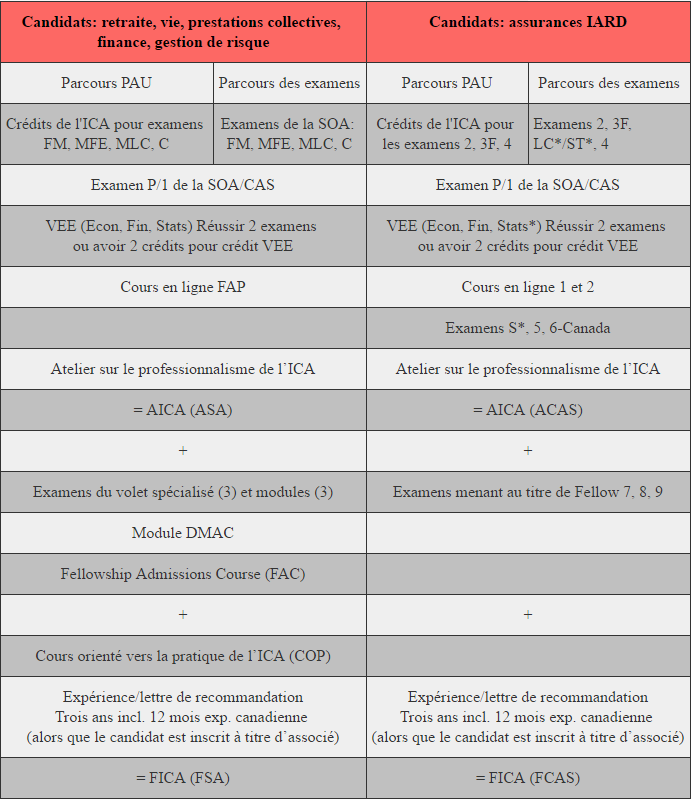
\includegraphics[width=0.92\textwidth]{tableau_ICA}
\caption{Cheminement professionnel en actuariat --- Grille fournie par Joseph Gabriel de l'Institut canadien des actuaires}
\end{figure}
\par
\end{center}

Note: Le nouvel examen S remplacera les examens LC/ST ainsi que le VEE \emph{Applied Statistical Methods} pour les candidats de la CAS.\vspace{\baselineskip}

Vous trouverez l'information quant aux cours qui permettent d'obtenir les accréditations d'examen de l'ICA dans votre \href{https://www.act.ulaval.ca/programmes-et-cours/premier-cycle/guide-de-letudiant/}{guide de l'étudiant}. Cette information se trouve généralement dans les dernières pages du document. Il est important de savoir que la CAS reconnaît les accréditation de l'ICA, mais que la SOA ne les reconnaît pas. Ainsi, un candidat qui obtient des accréditations pour certains examens peut obtenir les titres de Fellow de l'ICA et de la CAS mais, s'il est du côté de la SOA, il ne pourra pas devenir Fellow de la SOA --- il sera seulement Fellow de l'ICA.

\subsection*{Les crédits VEE}
\label{subsec:vee}
\addcontentsline{toc}{subsection}{Les crédits VEE}
Les crédits VEE (\emph{Validation by Educational Experience}) sont une composante nécessaire pour obtenir le titre d'Associé. Les VEE permettent de couvrir des sujets qui ne sont pas formellement testés lors des examens préliminaires. La CAS et la SOA ont deux VEE en commun: le VEE \emph{Corporate Finance} et le VEE \emph{Economics}. La SOA compte également le VEE \emph{Applied Statistical Methods}. Anciennement, la CAS comptait également ce troisième VEE, mais ils ont décidé de l'enlever suite à la création de l'Examen S.\vspace{\baselineskip}

Les crédits VEE peuvent être complétés en obtenant une note d'au moins B- dans certains cours du baccalauréat. Présentement, le cours qui permet d'obtenir le VEE \emph{Corporate Finance} est \textit{ACT-1006 Gestion du risque financier I}, alors que les cours qui permettent de compléter le VEE \emph{Economics} sont \textit{ECN-1000 Principes de microéconomie} \textbf{et} \textit{ECN-1010 Principes de macroéconomie}. Du côté de la SOA, on peut également obtenir le crédit VEE \emph{Applied Statistical Methods} avec une cote supérieure ou égale à B- dans les cours \textit{ACT-2003 Modèles linéaires en actuariat} \textbf{et} \textit{ACT-2010 Séries chronologiques}. Advenant le cas où vous n'auriez pas la cote minimale pour obtenir le crédit, vous devrez éventuellement compléter un cours en ligne sur le sujet du VEE en question, lequel sera suivi d'un examen.

\newpage
\subsection*{Les manuels d'étude}
\label{subsec:manuels}
\addcontentsline{toc}{subsection}{Les manuels d'étude}
En théorie, les livres de référence suggérés dans les syllabus\footnote{Le syllabus est un document officiel publié par la SOA pour chaque examen contenant une description du contenu de l'examen, des manuels à étudier et d'autres informations importantes.}{\tiny} des examens devraient suffir pour bien connaître la matière à l'examen. Par contre, il est sans doute préférable d'utiliser des manuels d'étude qui ont été écrits spécifiquement pour préparer les étudiants à ces examens. Il existe plusieurs \href{https://soa.org/education/exam-req/resources/edu-txt-manuals.aspx}{distributeurs} pour ces manuels d'études, mais il est souvent plus économique de les acheter usagés à des étudiants au sein du baccalauréat ou encore d'utiliser les versions électroniques de ces manuels qui sont en circulation sur le web. Il y a plusieurs auteurs qui rédigent des manuels d'étude pour les examens professionnels. Les plus réputés pour les examens préliminaires sont ceux de ASM et de ACTEX, bien qu'il en existe plusieurs autres (BPP, Guo, Mahler, etc.)\vspace{\baselineskip}

Les manuels d'étude de Marcel B. Finan, qui sont offerts gratuitement sur sa \href{http://faculty.atu.edu/mfinan/actuaries.html}{page web} sont également une bonne ressource (voir les liens sous l'onglet \emph{Study Guides}). Il faut toutefois se méfier des changements au syllabus depuis la dernière mise à jour de ces manuels.


\subsection*{Alternatives et compléments aux manuels}
\label{subsec:alternatives}
\addcontentsline{toc}{subsection}{Alternatives et compléments aux manuels}
Il existe quelques alternatives et compléments aux manuels d'étude qui ont été présentés ci-dessus. Par exemple, les sites \href{http://www.theinfiniteactuary.com/}{\emph{The Infinite Actuary}} et \href{https://www.coachingactuaries.com/}{\emph{Coaching Actuaries}} offrent des formations préparatoires sous forme de vidéos pour tous les examens préliminaires (et certains examens avancés dans le cas de \emph{The Infinite Actuary}). Ces ressources sont toutefois peu populaires auprès des étudiants du baccalauréat, puisqu'elles sont souvent dispendieuses.\vspace{\baselineskip}

Un complément incontournable aux manuels d'étude est le système dynamique de génération d'examens ADAPT. Ce système est offert par le site \href{https://www.coachingactuaries.com/}{\emph{Coaching Actuaries}} et comporte une énorme banque de questions pour chacun des examens préliminaires. Le fonctionnement de ADAPT est plutôt simple; on débute au niveau 0, le système génère des examens pour vous et, dépendamment de votre résultat à l'examen, votre niveau (\emph{Earned Level} en anglais) va augmenter. Le niveau de l'examen correspond à sa difficulté; plus il est élevé, plus il sera difficile. Vous pourrez également plus facilement voir quelles sont les sections de l'examen où vous avez le plus de difficulté et créer des quiz spécifiquement sur ces sections afin de vous améliorer. L'objectif est d'atteindre un niveau 7 (sans tricher --- évidemment), puisque les statistiques disponibles montrent qu'environ 90\% des gens qui ont atteint ce niveau ont réussi leur examen. En vous inscrivant avec votre adresse courriel universitaire, vous aurez droit à un rabais d'au moins 15\%. Voir cette \href{https://www.coachingactuaries.com/Students}{page} pour plus d'informations sur les rabais et ce \href{https://www.youtube.com/watch?v=ZBxLa2J5jhs}{vidéo} pour une brève présentation de ADAPT.

\newpage
\section*{Les examens préliminaires}
\label{sec:prelims}
\addcontentsline{toc}{section}{Les examens préliminaires}
Vous trouverez les dates importantes pour les examens préliminaires sur cette \href{https://www.soa.org/Education/Exam-Req/Exam-Day-Info/edu-2017-cbt-test-schedule.aspx}{page}. J'en profite également pour mentionner qu'en vous inscrivant avec votre adresse courriel universitaire, vous serez éligible à un rabais étudiant pour les examens MFE/3F, C/4 et MLC. Voir cette \href{https://soa.org/Education/Exam-Req/Syllabus-Study-Materials/Exam-and-Module-Fees.aspx}{page} pour plus de détails concernant les coûts d'inscription.


\subsection*{Examen P/1}
\label{subsec:examp}
\addcontentsline{toc}{subsection}{Examen P/1}
\href{https://www.soa.org/education/exam-req/edu-exam-p-detail.aspx}{L'examen P/1} a pour objectif de développer les notions essentielles de la théorie des probabilités dans le contexte de l'actuariat. La matière de cet examen est traitée dans le cours \textit{ACT-1002 Analyse probabiliste des risques actuariels}. Après avoir complété ce cours, des étudiants ont rapporté avoir étudié \textbf{environ} 50 à 100 heures pour l'examen P/1. Pour consulter les objectifs spécifiques de l'examen ainsi que d'autres informations, voir le \href{https://www.soa.org/Files/Edu/2017/edu-2017-01-p-syllabus.pdf}{syllabus}. Cet examen est d'une durée de 3h00 et comporte 30 questions à choix multiples (choix A, B, C, D, E). La SOA a publié \href{http://www.soa.org/Files/Edu/edu-exam-p-sample-quest.pdf}{326 questions} types pour cet examen, accompagnées du \href{http://www.soa.org/Files/Edu/edu-exam-p-sample-sol.pdf}{solutionnaire}.\vspace{\baselineskip}

À mon avis, le meilleur manuel d'étude pour l'examen P/1 est celui de ACTEX, écrit par Samuel Broverman. Le site \href{http://www.theinfiniteactuary.com/exams/1}{The Infinite Actuary} offre gratuitement quatre examens pratiques qui sont à peu près du même niveau que le véritable examen. C'est donc une excellente pratique pour vous. Enfin, une inscription à \href{https://www.coachingactuaries.com/}{ADAPT} peut également vous permettre de mieux déterminer si vous êtes prêt à faire l'examen et donc s'avérer un investissement très rentable.\vspace{\baselineskip}

Voici un exemple de plan d'étude pour l'examen P/1 (après avoir complété ACT-1002) :
\begin{enumerate}
\item Faire une lecture rapide du manuel ACTEX pour avoir une bonne vue d'ensemble de la matière à l'examen;
\item Relire les sections dans lesquelles vous avez plus de difficulté et faire des exercices jusqu'à devenir confortable;
\item Compléter les problèmes de la SOA en notant les problèmes que vous ne comprenez pas;
\item Relire les sections du manuel ACTEX pour combler les lacunes que vous aviez lorsque vous avez fait les problèmes de la SOA;
\item Débuter les examens pratiques dans le manuel ACTEX;
\item \textbf{Cinq jours avant l'examen :} faire deux examens par jour sur le site The Infinite Actuary;
\item \textbf{Trois jours avant l'examen :} refaire les problèmes que vous ne compreniez pas à l'étape trois et les problèmes ratés dans les examens pratiques;
\item \textbf{La journée avant l'examen :} faire une dernier survol léger de l'ensemble de la matière, relire ses notes et s'assurer de bien connaître les formules nécessaires.
\end{enumerate}
\vspace{\baselineskip}

Ce plan d'étude est seulement à titre indicatif et la majorité d'entre vous auront sans doute besoin de moins d'étude que ce qui y figure. Quelqu'un qui a bien réussi le cours ACT-1002 pourrait très bien faire une lecture rapide du manuel ACTEX, puis passer directement aux examens pratiques. Il faut garder en tête que les problèmes que vous devrez résoudre lors de l'examen P/1 seront moins compliqués que ceux du cours ACT-1002, mais la note de passage de cet examen est d'environ 70\% plutôt que d'être de 50\%. 

\newpage
\subsection*{Examen FM/2}
\label{subsec:examfm}
\addcontentsline{toc}{subsection}{Examen FM/2}
\href{https://www.soa.org/education/exam-req/edu-exam-fm-detail.aspx}{L'examen FM/2} traite des mathématiques financières et des produits dérivés. Les cours du baccalauréat en actuariat en lien avec cet examen sont \textit{ACT-1001 Mathématiques financières} et \textit{ACT-2011 Gestion du risque financier II} pour la partie produits dérivés. Après avoir complété le cours \textit{ACT-1001 Mathématiques financières}, des étudiants ont rapporté avoir étudié \textbf{environ} 75 à 175 heures pour l'examen FM/2. Pour consulter les objectifs spécifiques de l'examen ainsi que d'autres informations, voir le \href{https://www.soa.org/Files/Edu/2017/edu-2017-02-exam-fm-syllabus.pdf}{syllabus}. Cet examen est d'une durée de 3h00 et comporte 35 questions à choix multiples. La SOA a publié \href{https://www.soa.org/Files/Edu/2015/edu-2015-exam-fm-ques-theory.pdf}{133 questions} types sur les mathématiques financières ainsi que le \href{https://www.soa.org/Files/Edu/2015/edu-2015-exam-fm-sol-theory.pdf}{solutionnaire} et \href{https://www.soa.org/Files/Edu/edu-2014-10-exam-fm-ques.pdf}{64 questions} types sur les produits dérivés avec le \href{https://www.soa.org/Files/Edu/edu-2014-10-exam-fm-sol.pdf}{solutionnaire}.\vspace{\baselineskip} 

À mon avis, le meilleur manuel d'étude pour l'examen FM/2 est celui de ASM. Les explications sont extrêmement détaillées en plus d'avoir d'excellentes notes pour bien maîtriser la calculatrice BA II Plus, une compétence qui est très utile lors de l'examen. Personnellement, je n'avais pas utilisé ADAPT pour cet examen, puisque le manuel comporte déjà énormément de problèmes en plus d'examens pratiques qui sont comparables en difficulté au véritable examen. Vous trouverez, encore une fois, deux examens pratiques tout à fait gratuits sur le site \href{http://www.theinfiniteactuary.com/exams/2}{The Infinite Actuary}. La difficulté de ces deux examens pratiques est comparable au véritable examen.\vspace{\baselineskip} 

\textbf{Changements entrant en vigueur en juin 2017 :} Élimination des produits dérivés, à l’exception des swaps de taux d’intérêt. Ainsi, l'essentiel de la matière qui se trouve à l'examen sera traitée dans le cours \textit{ACT-1001 Mathématiques financières}.


\newpage
\subsection*{Examen MFE/3F}
\label{subsec:exammfe}
\addcontentsline{toc}{subsection}{Examen MFE/3F}
\href{https://www.soa.org/education/exam-req/edu-exam-mfe-detail.aspx}{L'examen MFE/3F} traite des modèles financiers et de leurs applications dans des contextes d'assurance et de gestion de risques. Les notions de produits dérivés, vues dans l'examen FM/2, seront utilisées comme base. Les cours du baccalauréat en lien avec cet examen sont \textit{ACT-2011 Gestion du risque financier II} et \textit{ACT-2009 Processus stochastiques} (dans une moindre mesure). Étant donné que le cours \textit{Gestion du risque financier II} sera véritablement mis à l'horaire pour la première fois à l'hiver 2017, il est difficile de déterminer le temps d'étude qui sera nécessaire une fois que ce cours aura été complété. Pour consulter les objectifs spécifiques de l'examen ainsi que d'autres informations, voir le \href{https://www.soa.org/Files/Edu/2016/edu-2016-11-mfe-syllabus.pdf}{syllabus}. Cet examen est d'une durée de 3h00 et comporte 30 questions à choix multiples. La SOA a publié \href{http://www.soa.org/files/edu/edu-exam-mfe-sample-quest-sol.pdf}{76 questions} types pour cet examen. Je vous conseille toutefois de ne pas trop perdre de temps sur ces questions, puisqu'elles ne sont pas représentatives de l'examen.\vspace{\baselineskip}

Pour ce qui est du manuel d'étude à utiliser, le plus populaire est celui de ASM, écrit par Abraham Weishaus. Toutefois, le \href{http://howardmahler.com/Teaching/MFE.html}{manuel} d'Howard Mahler est beaucoup apprécié par plusieurs et coûte seulement 50 USD en version électronique. Par contre, la principale critique au sujet de ce manuel est qu'il y a des lacunes au niveau des concepts plus avancés (mouvement brownien, lemme d'Itô, modèles pour les taux d'intérêt, etc.)\vspace{\baselineskip}

Pour cet examen, ADAPT est un outil extrêmement utile. Plusieurs personnes sur des forums de discussion disent que c'est probablement l'examen où les questions dans ADAPT sont le plus similaires aux questions lors du véritable examen. D'ailleurs, beaucoup d'étudiants rapportent qu'ils ont rencontré des questions dans l'examen formulées exactement de la même façon que des questions dans ADAPT. De plus, les examens pratiques du livre ASM ne sont pas tout à fait représentatifs du véritable examen et c'est pourquoi je recommande très fortement l'utilisation de ADAPT pour l'examen MFE/3F.\vspace{\baselineskip}

\textbf{Changements entrant en vigueur en juillet 2017 :} Les notions sur les produits dérivées qui étaient traitées dans l'examen FM/2 auparavant figureront désormais à l'examen MFE/3F. Les processus stochastiques sont éliminées du syllabus de l'examen; ceux-ci sont déplacés aux examens de fellowship pertinents. Pour un certain temps, le résultat de l’examen informatique ne sera pas connu immédiatement, le temps qu’une certaine expérience se développe.

\newpage
\subsection*{Examen C/4}
\label{subsec:examc}
\addcontentsline{toc}{subsection}{Examen C/4}
\href{https://www.soa.org/education/exam-req/edu-exam-c-detail.aspx}{L'examen C/4} est une introduction à la modélisation, à l'analyse de données statistiques dans un contexte d'affaires, à l'estimation et à la création d'intervalles de confiance pour les décisions basées sur les modèles statistiques. Les cours du baccalauréat en lien avec cet examen sont \textit{ACT-2001 Introduction à l'actuariat II}, \textit{ACT-2005 Mathématiques actuarielles IARD I} et \textit{ACT-2008 Mathématiques actuarielles IARD II}. Pour consulter les objectifs spécifiques de l'examen ainsi que d'autres informations, voir le \href{https://www.soa.org/Files/Edu/2017/edu-2017-02-exam-c-syllabus.pdf}{syllabus}. Cet examen est d'une durée de 3h30 et comporte 35 questions à choix multiples. La SOA a publié \href{http://www.soa.org/files/edu/edu-exam-c-sample-quest.pdf}{305 questions} types pour cet examen, accompagnées du \href{http://www.soa.org/files/edu/edu-exam-c-sample-sol.pdf}{solutionnaire}.\vspace{\baselineskip}

Pour ce qui est du manuel d'étude à utiliser, il y a principalement deux écoles de pensée qui s'affrontent. Le manuel le plus populaire est probablement celui de ASM, encore une fois écrit par Abraham Weishaus. Par contre, certaines personnes estiment que les explications sont souvent trop peu détaillées et qu'il est donc difficile de bien comprendre la matière avec ce manuel. À l'opposé, les gens qui utilisent le \href{http://howardmahler.com/Teaching/C.html}{manuel} d'Howard Mahler disent que l'auteur prend le temps de bien expliquer toute la théorie et qu'il présente un bon nombre d'astuces qui aident à gagner en rapidité au moment de l'examen. Le seul problème, c'est que le manuel de Mahler fait 5528 pages, contre 1282 pages pour le livre ASM (en excluant les examens pratiques --- il n'y a pas d'examens pratiques dans le livre de Mahler, ils doivent être achetés séparément). \vspace{\baselineskip}

Malgré tout, pour ceux qui ont déjà suivi les cours du baccalauréat qui traitent de la matière à l'examen C/4, le manuel ASM est sans doute suffisamment détaillé pour que vous atteigniez un niveau de préparation adéquat. Pour ceux qui voudraient faire l'examen avant de suivre les cours de mathématiques actuarielles IARD, je conseille d'utiliser le livre de Mahler.\vspace{\baselineskip}

Pour ce qui est des examens pratiques, plusieurs personnes sur les forums de discussion ont de très bons commentaires pour ceux d'\href{http://howardmahler.com/Teaching/C.html}{Howard Mahler}, vendus séparément de son livre. Bien qu'ils semblent généralement être considérés comme difficiles, ces examens pratiques permettent vraiment de bien appliquer la matière et d'établir des connexions entre les différents sujets. À l'opposé, plusieurs ont tendance à dire que ADAPT n'est pas un bon outil pour cet examen, puisque la formulation des questions n'est pas représentative du véritable examen. 

%\subsection*{Examen MLC (SOA)}
%\label{subsec:exammlc}
%\addcontentsline{toc}{subsection}{Examen MLC (SOA)}



%\subsection*{Examen S (CAS)}
%\label{subsec:exams}
%\addcontentsline{toc}{subsection}{Examen S (CAS)}


\newpage
\section*{Autres informations}
\label{sec:autres}
\addcontentsline{toc}{section}{Autres informations}

\subsection*{Liens utiles}
\label{subsec:liens}
\addcontentsline{toc}{subsection}{Liens utiles}
Pour ceux qui sont intéressés par le domaine de la finance ou qui cherchent à étendre leurs champs d'expertise, la désignation professionnelle CFA peut être une très bonne option. C'est sans doute la désignation du monde de la finance qui est la plus reconnue à l'international et un nombre considérable d'actuaires la possèdent. Afin d'obtenir cette désignation, l'on doit passer trois examens (\emph{Level I, II} et \emph{Level III}) et avoir quatre ans d'expérience pertinente dans le milieu de la finance. Concernant l'expérience demandée, il est difficile de connaître les critères exactes du CFA Institute mais, généralement, il faut qu'une majorité du temps de travail de ces quatre années soit relié à la gestion d'actifs au sens large. Les examens \emph{Level II \emph{et} Level III} sont offerts seulement une fois par année, le premier samedi du mois de juin, alors que le \emph{Level I} est également offert au mois de décembre. Pour plus d'informations, consulter la page du \href{https://www.cfainstitute.org/Pages/index.aspx}{\emph{CFA Institute}}. Vous pouvez également lire l'article \href{http://blog.coachingactuaries.com/why-would-actuaries-consider-getting-a-cfa/}{\emph{Why would Actuaries consider getting a CFA?}}.\vspace{\baselineskip}

Ceux qui sont intéressés par l'informatique et le \emph{data science} pourront s'informer au sujet de la création du \href{http://www.casact.org/press/index.cfm?fa=viewArticle&articleID=3083}{CAS Institute}.\vspace{\baselineskip} 

\newpage
\subsection*{Changements aux prérequis pour devenir Associé}
\label{subsec:changeasa}
\addcontentsline{toc}{subsection}{Changements aux prérequis pour devenir Associé}
La SOA est présentement en processus de restructuration des prérequis pour devenir Associé. Ils ont fait une annonce officielle à la fin du mois de juin pour préciser davantage la nouvelle structure, qui devrait être effective à partir du 1ier juillet 2018. Le plus gros changement est l’ajout de deux nouveaux examens, mais ce sont toutes les composantes qui vont être modifiées.\vspace{\baselineskip} 

\textbf{Voici les éléments clés de l’annonce de juin :}
\begin{itemize}
\item Ajout de la tarification et des méthodes de réserve à l’examen C/4
\item Tous les concepts liés aux produits dérivés seront désormais dans l'examen MFE/3F (à l'exception des swaps de taux d'intérêt)
\item Retrait des concepts plus avancés de l’examen MFE/3F (processus stochastiques, mouvement brownien, modèles de taux d’intérêt, etc.)
\item Ajout d’un examen sur les statistiques appliquées – \emph{Statistics for Risk Modeling}  
\item Ajout d’un examen sur l’analyse de données - \emph{Predictive Analytics}
\item Le VEE finance comptera une partie sur la comptabilité 
\end{itemize}
\vspace{\baselineskip} 

La CAS a déjà annoncé qu’elle reconnaîtrait le nouveau format des examens FM/2 et MFE/3F à partir de l’été 2017, au moment où les modifications prendront effet pour ces deux examens. Je tenterai de vous tenir au courant des développements dans les prochains mois. N’hésitez pas à communiquer avec moi s’il y a quoi que ce soit.\vspace{\baselineskip} 

Quelques liens supplémentaires :
\begin{enumerate}
\item \href{https://www.soa.org/Education/General-Info/2016-asa-cera-curriculum-changes.aspx}{Annonce du 28 juin par la SOA}
\item \href{https://soa.qualtrics.com/CP/File.php?F=F_0TDd9bj143TrCW9}{Annonce préliminaire de la SOA (janvier 2016)}
\item \href{https://www.soa.org/Education/General-Info/2016-transition-rules-asa-candidated.aspx}{L’équivalence des examens actuels dans le système à venir}
\item \href{http://www.casact.org/press/index.cfm?fa=viewArticle&articleID=3273}{Annonce de la CAS pour le nouveau format de FM/2 et MFE/3F}
\end{enumerate}

\begin{figure}[hp]
\begin{center}
\textbf{Changements aux prérequis pour devenir Associé}\par\medskip
\end{center}
\hfill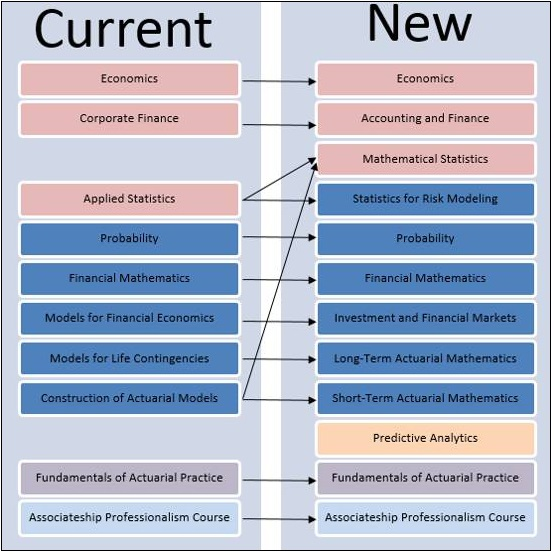
\includegraphics{Change_ASA}\hspace*{\fill}
\caption{Équivalences des examens actuels dans le système à venir}
\end{figure}
\par

\newpage
\section*{Annexes}
\label{sec:annexes}
\addcontentsline{toc}{section}{Annexes}
\subsection*{Procédure pour les crédits VEE (SOA et CAS)}
\label{subsec:vee}
\addcontentsline{toc}{subsection}{Procédure pour les crédits VEE (SOA et CAS)}
Une fois que vous avez complété le ou les cours nécessaires pour obtenir votre crédit VEE, vous devez faire la demande pour que celui-ci soit ajouté à votre dossier.\footnote{Vous pouvez trouver des informations concernant les cours qui permettent d'obtenir les crédits VEE dans votre \href{https://www.act.ulaval.ca/programmes-et-cours/premier-cycle/guide-de-letudiant/}{guide étudiant} ou encore sur cette \href{https://soa.org/Education/Exam-Req/Instructions-for-VEE-Directory.aspx}{page de la SOA}.} La procédure est la même pour les candidats de la SOA et les candidats de la CAS. Elle comporte principalement deux étapes: remplir le formulaire de la SOA et acheminer le relevé de notes de l'Université Laval au bureau d'administration des VEE de la SOA.\vspace{\baselineskip} 

\begin{enumerate}
\item \textbf{Remplir le formulaire de la SOA}
\begin{itemize}
\item Se rendre sur la \href{https://soa.org/education/exam-req/edu-vee.aspx}{page d'information sur les VEE}. 
\item Cliquer sur le type d'application pour le VEE qui vous intéresse (\textit{Apply online for VEE Economics Credit}, \textit{Apply online for VEE Corporate Finance Credit} ou \textit{Apply online for VEE Applied Statistics Credit}.
\item Entrer vos informations personnelles et cliquer sur \textit{Select School / University} pour pouvoir accéder à la liste de cours qui sont approuvés pour les VEE.
\item Sélectionner le pays et la province, puis sélectionner l'Université Laval. La liste de cours devrait apparaître. \item Cibler la ligne du cours que vous avez complété et entrer la cote obtenue et la date à laquelle vous avez terminé ce cours. 
\item Cliquer sur \textit{Select} (complètement à gauche de la ligne). Il vous reste ensuite simplement à payer le montant qui sera indiqué.
\end{itemize}\vspace{\baselineskip}
\item \textbf{Acheminer le relevé de notes de l'Université Laval à la SOA}
\begin{itemize}
\item Se rendre sur la \href{https://www.reg.ulaval.ca/cms/DemDoc/releveNotes}{page du Bureau du registraire} pour les relevés de notes.
\item Remplir le formulaire \textbf{REG-910-RN}. Le relevé de notes doit être acheminé au bureau d'administration des VEE de la SOA. L'adresse se trouve sur cette \href{https://soa.org/education/exam-req/course-info/edu-vee-applying-process.aspx}{page}.
\item Acheminer ce formulaire au bureau du registraire en suivant les indications sur la page concernant les relevés de notes.
\end{itemize}
\end{enumerate}


\newpage
\subsection*{Procédure pour l'inscription aux examens préliminaires}
\label{subsec:inscriptionexams}
\addcontentsline{toc}{subsection}{Procédure pour l'inscription aux examens préliminaires}
La procédure pour l'inscription aux examens préliminaires est la même pour les candidats de la CAS et les candidats de la SOA. Elle comporte principalement deux étapes : l'inscription à l'examen sur le site de la SOA et fixer la date sur le site de Prometric.\footnote{Cette dernière étape est omise si vous faites l'examen papier.}\vspace{\baselineskip} 

\begin{enumerate}
\item \textbf{Inscription à l'examen sur le site de la SOA}
\begin{itemize}
\item Se rendre sur la \href{https://www.soa.org/Education/Exam-Req/Registration/edu-registration.aspx}{page d'inscription}. 
\item Sélectionner l'examen de votre choix. Si ce n'est pas déjà fait, vous devrez vous créer un compte sur le site de la SOA.
\item Payer le montant indiqué.
\item Vous recevrez une lettre de confirmation de votre commande par courriel, qui contient notamment votre numéro de candidat.
\end{itemize}\vspace{\baselineskip}

\item \textbf{Fixer la date sur le site de Prometric}
\begin{itemize}
\item Vous recevrez un deuxième courriel (\textit{Letter of confirmation}) qui vous informera de vous inscrire sur le site de Prometric. Ce courriel est envoyé environ 3 à 5 jours ouvrables après avoir payé pour l'examen.
\item Suivre les instructions qui figurent dans ce courriel afin de fixer une date pour votre examen. Pour ce faire, vous devrez utiliser votre numéro d'éligibilité qui figure dans ce second courriel.
\end{itemize}
\end{enumerate}

\newpage
\subsection*{Foire aux questions}
\label{subsec:faq}
\addcontentsline{toc}{subsection}{Foire aux questions}
Cette section est en construction. Envoyez-moi vos questions par rapport aux examens professionnels, au cheminement en actuariat ou sur tout autre sujet que vous jugerez pertinent et je mettrai à jour cette section du document avec les réponses à vos questions. Vous pouvez me rejoindre à l'adresse courriel suivante: \emph{antoine.beaupre.1@ulaval.ca}.

\end{document}